\documentclass[12pt]{article}

% Solutions toggle
\newif\ifsolutions
\solutionsfalse
%% \solutionstrue

% ASSIGNMENT NUMBER
\newcommand{\hwnumber}{7}
\newcommand{\booksection}{}
\newcommand{\duedate}{}
% -------------

%%% Packages
\usepackage[margin=1in, footskip=24pt, headheight=24pt]{geometry}
\usepackage{amsmath, amssymb, amsthm, graphicx}
\usepackage{mathtools}
\DeclarePairedDelimiter\ceil{\lceil}{\rceil}
\DeclarePairedDelimiter\floor{\lfloor}{\rfloor}
\usepackage[colorlinks, urlcolor=blue]{hyperref}
\usepackage{color}
\usepackage{comment}
\usepackage{enumerate}
\usepackage{lastpage}
\usepackage{multirow, multicol}
\usepackage{tikz}
\usetikzlibrary{matrix,decorations.text,decorations.pathmorphing,decorations.markings,arrows,calc,shapes.geometric,patterns,shadows,intersections,decorations.markings,decorations.pathreplacing,decorations.pathreplacing,backgrounds,angles,quotes}
\usepackage{pgfplots}
\pgfplotsset{compat=1.16}

\usepackage{fancyhdr}

\pagestyle{fancy}
%% \renewcommand{\familydefault}{\sfdefault}

\newcommand{\R}{\mathbb{R}}
\newcommand{\ddx}{\frac{d}{dx}}

\global\long\def\V#1{\boldsymbol{#1}} %vector
\global\long\def\M#1{\boldsymbol{#1}} %matrix

\global\long\def\D#1{\Delta#1} %\D{t} for time step size
\global\long\def\d#1{\delta#1} %\d{t} for small increment

\global\long\def\norm#1{\left\Vert #1\right\Vert }
\global\long\def\abs#1{\left|#1\right|}

\global\long\def\grad{\M{\nabla}}
\global\long\def\av#1{\left\langle #1\right\rangle }

% HEADER MACROS
\newcommand{\term}{Spring 2022 \& 2023}
\newcommand{\coursename}{Intro Math Modeling}
\newcommand{\coursenumber}{MATH-UA 251}
\newcommand{\course}{\coursename \ (\coursenumber)}

\fancyhead[RO]{\term}
\fancyhead[LO]{\course}
% -------------

%%% Theorem Styles
\theoremstyle{definition}
\newtheorem{ex}{Exercise}

%%%%%%%%%%%%%%%%%%%%%%%% Solutions %%%%%%%%%%%%%%%%%%%%%%%%%%%%%
% \begin{solution} and \begin{answerspace} must be at the beginning of the line.
% Doesn't work inside the \myversions command. Use if statements instead.
% No underscores in comment names

\ifsolutions
\newenvironment{solution}{\color{blue}}{} \excludecomment{answerspace} \newenvironment{notes}{\color{red} \noindent Grading Notes:}{}
\else
\excludecomment{notes} \excludecomment{solution} \includecomment{answerspace} 
\fi
%%%%%%%%%%%%%%%%%%%% End Solutions %%%%%%%%%%%%%%%%%%%%%%%e}


\begin{document}
% HEADER
\begin{center}
%% \ifsolutions
%%   \textbf{\Large Homework \hwnumber\ - \booksection\ (Solutions)}\\
%% \else
%%   \textbf{\Large Homework \hwnumber\ - \booksection}\\
%% \fi
\ifsolutions
  \textbf{\Large Homework \hwnumber\ (Solutions)}\\
\else
  \textbf{\Large Homework \hwnumber}\\
\fi
\vspace{12pt}
Due date: someday, sometime! \duedate

Submit on NYU Brightspace.
\end{center}

%% \noindent Please give complete, well-written solutions to the following exercise. Provide sufficient justification and explanation for a classmate who has not worked on the exercise to understand your solution.


\begin{ex}

  Consider a particle of mass $m$ and electric charge $q$, initially at rest (zero velocity, $v(0)=0$), placed in a unidirectional potential $\psi(x)=-E_0qx\sin(\omega t)$. Assume that the particle experiences a spatially uniform electric force given by (for this one-dimensional system) as $F_E=-\partial\psi/\partial x$, and a nonlinear drag force in the from $F_D=\delta v^3$.

  \begin{enumerate}[(i)]
  \item Use the Newton's second law to write the equation of motion for the particle's velocity.
  \item Take $\tilde{t}=\omega t$ and $\tilde{v}=v/v_0$ (with $v_0$ to be determined) as the normalized, dimensionless, time and velocity. Substitute into the equation of motion and find $v_0$, so that there remains only one dimensionless group and it is the coefficient of $\tilde{v}^3$.
  \item Solve the obtained dimensionless equation of motion for $\tilde{v}(t)$ using a regular first-order perturbation method: $\tilde{v}(t)=\tilde{v}^{(0)}(t)+\epsilon \tilde{v}^{(1)}(t)+O(\epsilon^2)$. Clearly, and with details, show how you find the zeroth-order and first-order systems, and the solution procedure. You might need the trigonometric identities $\cos^3(t)=\tfrac{1}{4}(\cos(3t)+3\cos(t))$ and $\cos^2(t)=\tfrac{1}{2}(\cos(2t)+1)$.
  \item For $\epsilon=0.05$, solve the problem using Euler's method with $\Delta\tilde{t}=0.01\gamma$ and a total time of $10\gamma$, where $\gamma=2\pi$ is the dimensionless period. Plot the solution $\tilde{v}$ obtained using the regular perturbation and the one from the Euler's method versus $\tilde{t}/\gamma$ in one figure. How do these two solutions compare? Discuss. Hint: If done properly, you should see from the Euler's method that the particle's velocity oscillates and after a few cycles, reaches to a harmonic solution with zero time-average, i.e., the particle should not move on average over a cycle when the oscillation is harmonic.
  \item Solve the equation of motion using two-timing. Let $\tau=\tilde{t}$ and $T=\epsilon\tilde{t}$ be the fast and slow times. Investigate what caused the problems, if any, in the regular perturbation theory. Perhaps some terms on the right hand side of the first-order system? Get rid of them by a suitable choice of the involved constant (or a relation between the constant and its derivative). Hint: at some point you encounter the integral $\int{(2x^3+3x)^{-1}}dx$ which you can evaluate by partial fractions. Plot the two-timing and numerical $\tilde{v}$ versus $\tilde{t}/\gamma$ in one figure. Use the same parameters as the ones in part (iv). Discuss the new results.
  \end{enumerate}
  
\noindent\textbf{\textcolor{red}{notes:} }Show all of the steps of your work. Solutions without details of the work and interpretation of the results will not receive full credits. No result can be directly taken from the notes or elsewhere. Submit your code (commented) as well.

\begin{solution}
  \begin{enumerate}[(i)]\setlength{\itemsep}{0pt}
  \item There are only two forces involved, and the equation of motion is
    \textcolor{purple}{$$m\frac{dv}{dt}=E_0q\sin(\omega t)-\delta v^3.$$}
  \item Substitute $t=\tilde{t}/\omega$ and $v=v_0\tilde{v}$ into the equation of motion yields
    $$m\omega v_0\frac{d\tilde{v}}{d\tilde{t}}=E_0q\sin{\tilde{t}}-\delta v_0^3\tilde{v}^3\Rightarrow\frac{d\tilde{v}}{d\tilde{t}}=\frac{E_0q}{m\omega v_0}\sin{\tilde{t}}-\frac{\delta v_0^3}{m\omega v_0}\tilde{v}^3.$$
    If we take \textcolor{purple}{$v_0=E_0q/(m\omega)$}, the dimensionless equation of motion simplifies to
    \textcolor{purple}{$$\frac{d\tilde{v}}{d\tilde{t}}=\sin{\tilde{t}}-\epsilon\tilde{v}^3,$$}
    where \textcolor{purple}{$\epsilon=\delta v_0^2/(m\omega)$.}
  \item We drop the $\sim$ sign for simplicity of the notation. Substituting $v(t)=v^{(0)}(t)+\epsilon v^{(1)}(t)$ into the equation of motion yields
    $$\dot{v}^{(0)}+\epsilon\dot{v}^{(1)}=\sin(t)-\epsilon\left(v^{(0)}+\epsilon v^{(1)}\right)^3.$$
    We collect the terms with common power of $\epsilon$: $\dot{v}^{(0)}=\sin(t)$ and $\dot{v}^{(1)}=-\left(v^{0}\right)^3$. The initial condition is given as $v(0)=v^{(0)}(0)+\epsilon v^{(1)}(0)=0\Rightarrow v^{(0)}(0)=0,v^{(1)}(0)=0$. Therefore the zeroth and first order systems can be expressed as
    \begin{align*}
      &O(\epsilon^0):\quad \dot{v}^{(0)}=\sin(t),\;v^{(0)}(0),\\
      &O(\epsilon^1):\quad \dot{v}^{(1)}=-\left(v^{0}\right)^3,\;v^{(1)}(0).
    \end{align*}
    \begin{itemize}
    \item zeroth order, $O(\epsilon^0)$
      \begin{align*}
        &\frac{dv^{(0)}}{dt}=\sin(t)\Rightarrow v^{(0)}=-\cos(t)+A,\\
        &v^{(0)}(0)=0\Rightarrow A=1,\\
        &v^{(0)}(t)=1-\cos(t).
      \end{align*}
    \item first order, $O(\epsilon^1)$
      \begin{align*}
        \frac{dv^{(1)}}{dt}&=-\left(v^{(0)}\right)^3=(\cos(t)-1)^3,\\
        \Rightarrow\frac{dv^{(1)}}{dt}&=\cos^3(t)-3\cos^2(t)+3\cos(t)-1\\
        &=\tfrac{1}{4}(\cos(3t)+3\cos(t))-\tfrac{3}{2}(\cos(2t)+1)+3\cos(t)-1\\
        &=\tfrac{1}{4}\cos(3t)-\tfrac{3}{2}\cos(2t)+\tfrac{15}{4}\cos(t)-\tfrac{5}{2}.
      \end{align*}
      To find $v^{(1)}$, integrate the above expression once:
      $$v^{(1)}=\tfrac{1}{12}\left[\sin(3t)-9\sin(2t)+45\sin(t)\right]-\tfrac{5}{2}t+B,$$
      where the initial condition $v^{(1)}(0)=0$ gives $B=0$. Therefore, the first-order term is
      $$v^{(1)}(t)=\tfrac{1}{12}\left[\sin(3t)-9\sin(2t)+45\sin(t)\right]-\tfrac{5}{2}t.$$
    \end{itemize}

    The first-order regular perturbation solution is\textcolor{purple}{
      $$v(t)=1-\cos(t)+\tfrac{1}{12}\epsilon\left[\sin(3t)-9\sin(2t)+45\sin(t)\right]-\tfrac{5}{2}\epsilon t.$$}

  \item The Euler's method can be written as
    \textcolor{purple}{$$v_{i+1}=v_i+\Delta t\left[\sin(t_i)-\epsilon v_i^3\right],$$}%
    which is implemented in the accompanying code chargedParticle.py. \autoref{Figure_reg} shows a comparison between the regular perturbation and numerical solution. The numerical solution indicates that the particle is initially at rest; then it moves back and forth, in response to the electric field, and, after a few cycles, reaches to the harmonic behavior. The particle, as expected, does not move on average. The regular perturbation solution, however, does not provide a proper prediction. We see that it is initially aligned with the Euler's solution but veers off eventually. This is unphysical given the symmetry of the system. The problematic term in the perturbation solution is $-\tfrac{5}{2}\epsilon t$ which grows in magnitude indefinitely as $t\to\infty$. This term could be avoided if there was no constant in the right hand side of $dv^{(1)}/dt$ equation. It makes sense since it indicates a constant acceleration. We will take care of it by two-timing.
    
    \begin{figure}[h]
    \centering
    \resizebox{0.4\textwidth}{!}{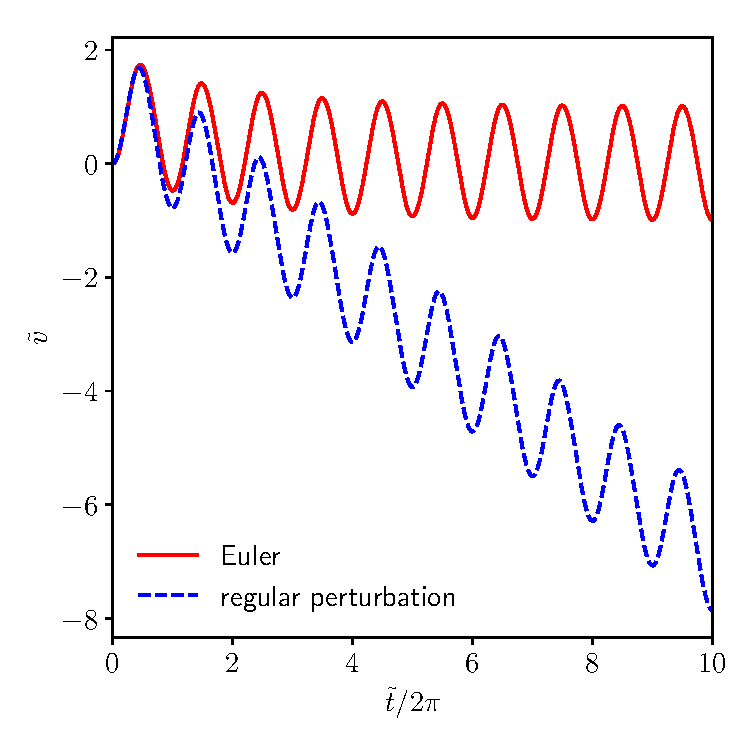
\includegraphics{HW7_reg.pdf}}
    \caption{particle's velocity versus time for numerical and regular perturbation solutions.}
    \label{Figure_reg}
    \end{figure}

  \item We use the chain rule to write $dv/dt$ in terms of derivative with respect to $\tau=t$ and $T=\epsilon t$:
    $$\frac{dv}{dt}=\frac{\partial v}{\partial \tau}\frac{d\tau}{dt}+\frac{\partial v}{\partial T}\frac{dT}{dt}=\frac{\partial v}{\partial \tau}+\epsilon\frac{\partial v}{\partial T}.$$
    Now, substituting the two-timing perturbation expression, i.e.,
    $$v(t)=v^{(0)}(\tau,T)+\epsilon v^{(1)}(\tau,T)$$
    results in
    $$\frac{dv}{dt}=\frac{\partial v^{(0)}}{\partial\tau}+\epsilon\frac{\partial v^{(1)}}{\partial\tau}+\epsilon\left[\frac{\partial v^{(0)}}{\partial T}+\epsilon\frac{\partial v^{(1)}}{\partial T}\right]=\frac{\partial v^{(0)}}{\partial\tau}+\epsilon\left[\frac{\partial v^{(1)}}{\partial\tau}+\frac{\partial v^{(0)}}{\partial T}\right]+O(\epsilon^2).$$
  \end{enumerate}
  Therefore, one can write the equation of motion as
  $$\frac{\partial v^{(0)}}{\partial\tau}+\epsilon\left[\frac{\partial v^{(1)}}{\partial\tau}+\frac{\partial v^{(0)}}{\partial T}\right]=\sin(\tau)-\epsilon\left(v^{(0)}\right)^3.$$

  \begin{itemize}
  \item zeroth order, $O(\epsilon^0)$

    We have
    $$\frac{\partial v^{(0)}}{\partial\tau}=\sin(\tau)\Rightarrow v^{(0)}=-\cos(\tau)+A(T).$$
    Note that the ``constant'' $A$ is a function of slow time $T$.
  \item first order, $O(\epsilon^1)$

    The first-order differential equation is
    $$\frac{\partial v^{(1)}}{\partial\tau}+\frac{\partial v^{(0)}}{\partial T}=-\left(v^{(0)}\right)^3\Rightarrow\frac{\partial v^{(1)}}{\partial\tau}=-A'+(\cos(\tau)-A)^3,$$
    where $A'=dA/dT$. We expand the right hand side to look for the problematic terms:
    \begin{align*}
      \frac{\partial v^{(1)}}{\partial\tau}&=-A'+\cos^3(\tau)-3A\cos^2(\tau)+3A^2\cos(\tau)-A^3\\
      &=-A'+\tfrac{1}{4}(\cos(3\tau)+3\cos(\tau))-\tfrac{3}{2}A(\cos(2\tau)+1)+3A^2\cos(\tau)-A^3\\
      &=-A'+\tfrac{1}{4}\cos(3\tau)-\tfrac{3}{2}A\cos(2\tau)+3\left(A^2+\tfrac{1}{4}\right)\cos(\tau)-\tfrac{3}{2}A-A^3.
    \end{align*}
    To avoid the constant acceleration terms, we let
    \begin{align*}
      &-A'-\tfrac{3}{2}A-A^3=0\Rightarrow \frac{dA}{dT}=-\tfrac{3}{2}A-A^3\Rightarrow \frac{dA}{2A^3+3A}=-\tfrac{1}{2}dT,\\
      &\Rightarrow \int{\frac{dA}{2A^3+3A}}=\tfrac{1}{6}\ln\left(\frac{A^2}{2A^2+3}\right)=-\tfrac{1}{2}T+B\Rightarrow \ln\left(\frac{A^2}{2A^2+3}\right)=-3T+6B\\
      &\Rightarrow \frac{2A^2+3}{A^2}=e^{-6B}e^{3T}\Rightarrow A^2=\frac{3}{Ke^{3T}-2}\Rightarrow A=\sqrt{\frac{3}{Ke^{3T}-2}}.
    \end{align*}
  \end{itemize}
    To find $K$ we use the initial condition $v(0)=0$ which yields $v^{(0)}(0,0)=0$ and $v^{(1)}(0,0)=0$. Applying the initial condition on the zeroth-order term gives
    $$v^{(0)}(0,0)=-\cos(0)+A(0)=-1+\sqrt{\frac{3}{K-2}}=0\Rightarrow K=5.$$
    The first-order solution is obtained by integrating the $dv^{(1)}/dt$ expression above (note that the non-oscillatory terms are now vanished):
    $$v^{(1)}=\tfrac{1}{12}\sin(3\tau)-\tfrac{3}{4}A\sin(2\tau)+3\left(A^2+\tfrac{1}{4}\right)\sin(\tau)+C,$$
    where $C=0$ from the initial condition $v^{(1)}(0,0)=0$.

    Finally, the first-order solution can be written as\textcolor{purple}{
      $$v(t)=-\cos(t)+A+\tfrac{1}{12}\sin(3t)-\tfrac{3}{4}A\sin(2t)+3\left(A^2+\tfrac{1}{4}\right)\sin(t),$$}
    where\textcolor{purple}{
    $$A=\sqrt{\frac{3}{5e^{3\epsilon t}-2}}.$$}%
    \autoref{Figure_twoTiming} shows a comparison between the numerical and two-timing solutions. The two-timing method does a great job in predicting the system behavior.
    
  \begin{figure}[t]
    \centering
    \resizebox{0.4\textwidth}{!}{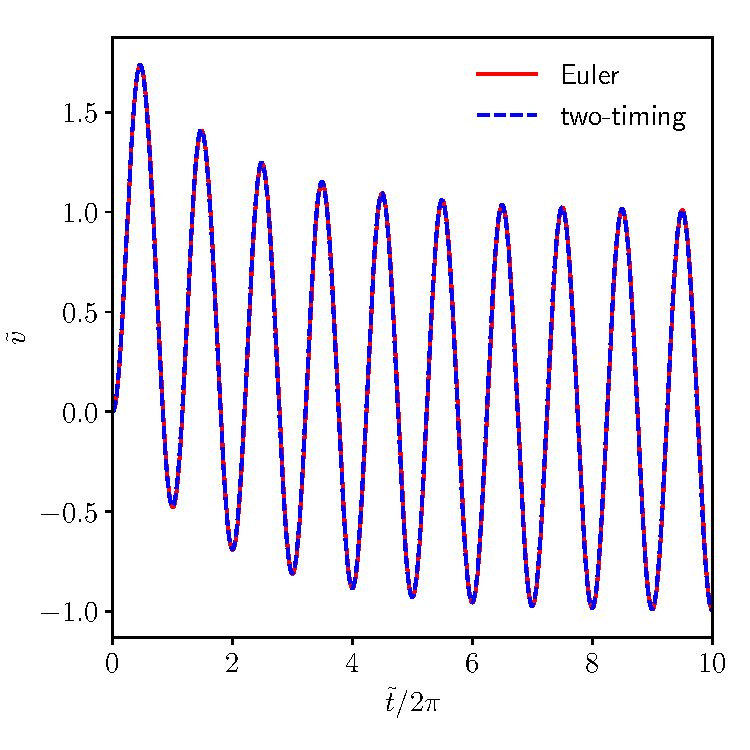
\includegraphics{HW7_twoTiming.pdf}}
    \caption{particle's velocity versus time for numerical and two-timing perturbation solutions.}
    \label{Figure_twoTiming}
    \end{figure}
\end{solution}
\end{ex}


\end{document}
